\documentclass{article}[11pt,paper=A4, margin=1cm]
% Language setting
% Replace `english' with e.g. `spanish' to change the document language
\usepackage[german]{babel}

% Set page size and margins
% Replace `letterpaper' with `a4paper' for UK/EU standard size
\usepackage[letterpaper,top=2cm,bottom=2cm,left=3cm,right=3cm,marginparwidth=1.75cm]{geometry}% Useful packages
\usepackage{amsmath}
\usepackage{amsfonts} 
\usepackage{amssymb}
\usepackage{mathtools}
\usepackage{graphicx}
\usepackage[colorlinks=true, allcolors=blue]{hyperref}
\usepackage{float}
\usepackage{multicol}
\usepackage{xcolor}
\usepackage{amsfonts}
\usepackage[utf8]{inputenc}
\usepackage{pgfplots}
\usepackage{listings}
\usepackage[linewidth=1pt]{mdframed}
\usepackage{lipsum}
\usepackage{subfiles} % Best loaded last in the preamble
\usepackage[backend=biber]{biblatex}
\usepackage{csquotes}
%=================================
%Code Formatting
\usepackage{listings}

\definecolor{dkgreen}{rgb}{0,0.6,0}
\definecolor{gray}{rgb}{0.5,0.5,0.5}
\definecolor{mauve}{rgb}{0.58,0,0.82}
\definecolor{backcolour}{rgb}{0.95,0.95,0.92}


\lstset{frame=tb,
    language=java,
    aboveskip=3mm,
    belowskip=3mm,
    showstringspaces=false,
    columns=flexible,
    basicstyle={\small\ttfamily},
    numbers=none,
    numberstyle=\tiny\color{black},
    backgroundcolor=\color{backcolour},
    keywordstyle=\color{blue},
    commentstyle=\color{dkgreen},
    stringstyle=\color{mauve},
    breaklines=true,
    breakatwhitespace=true,
    tabsize=2,
    numbersep=5pt,
    numbers=left
   }


% For labeling sub figures
\usepackage{subfigure}

\addbibresource{PE_Lab.bib}
\pgfplotsset{compat=1.18}

%=================PathVariable==============================
\def\cubeControllerFile{..//UnityProj/Assets/Scripts/CubeController.cs}
\def\lineControllerFile{..//UnityProj/Assets/Scripts/LineController.cs}
\def\lineJuliaFile{..//UnityProj/Assets/Scripts/LineJulia.cs}
\def\ropeSpawnFile{..//UnityProj/Assets/Scripts/RopeSpawn.cs}
\def\swingJuliaFile{..//UnityProj/Assets/Scripts/SwingJulia.cs}
\def\ropeSpawnFile{..//UnityProj/Assets/Scripts/RopeSpawn.cs}
\def\swingRomeoFile{..//UnityProj/Assets/Scripts/SwingRomeo.cs}




\title{Semesterprojekt Physik Engines}
\author{Kim Lan Vu, Michel Steiner, Asha Schwegler}




\begin{document}

\maketitle
\begin{figure}[H]
    \begin{center}
        \centerline{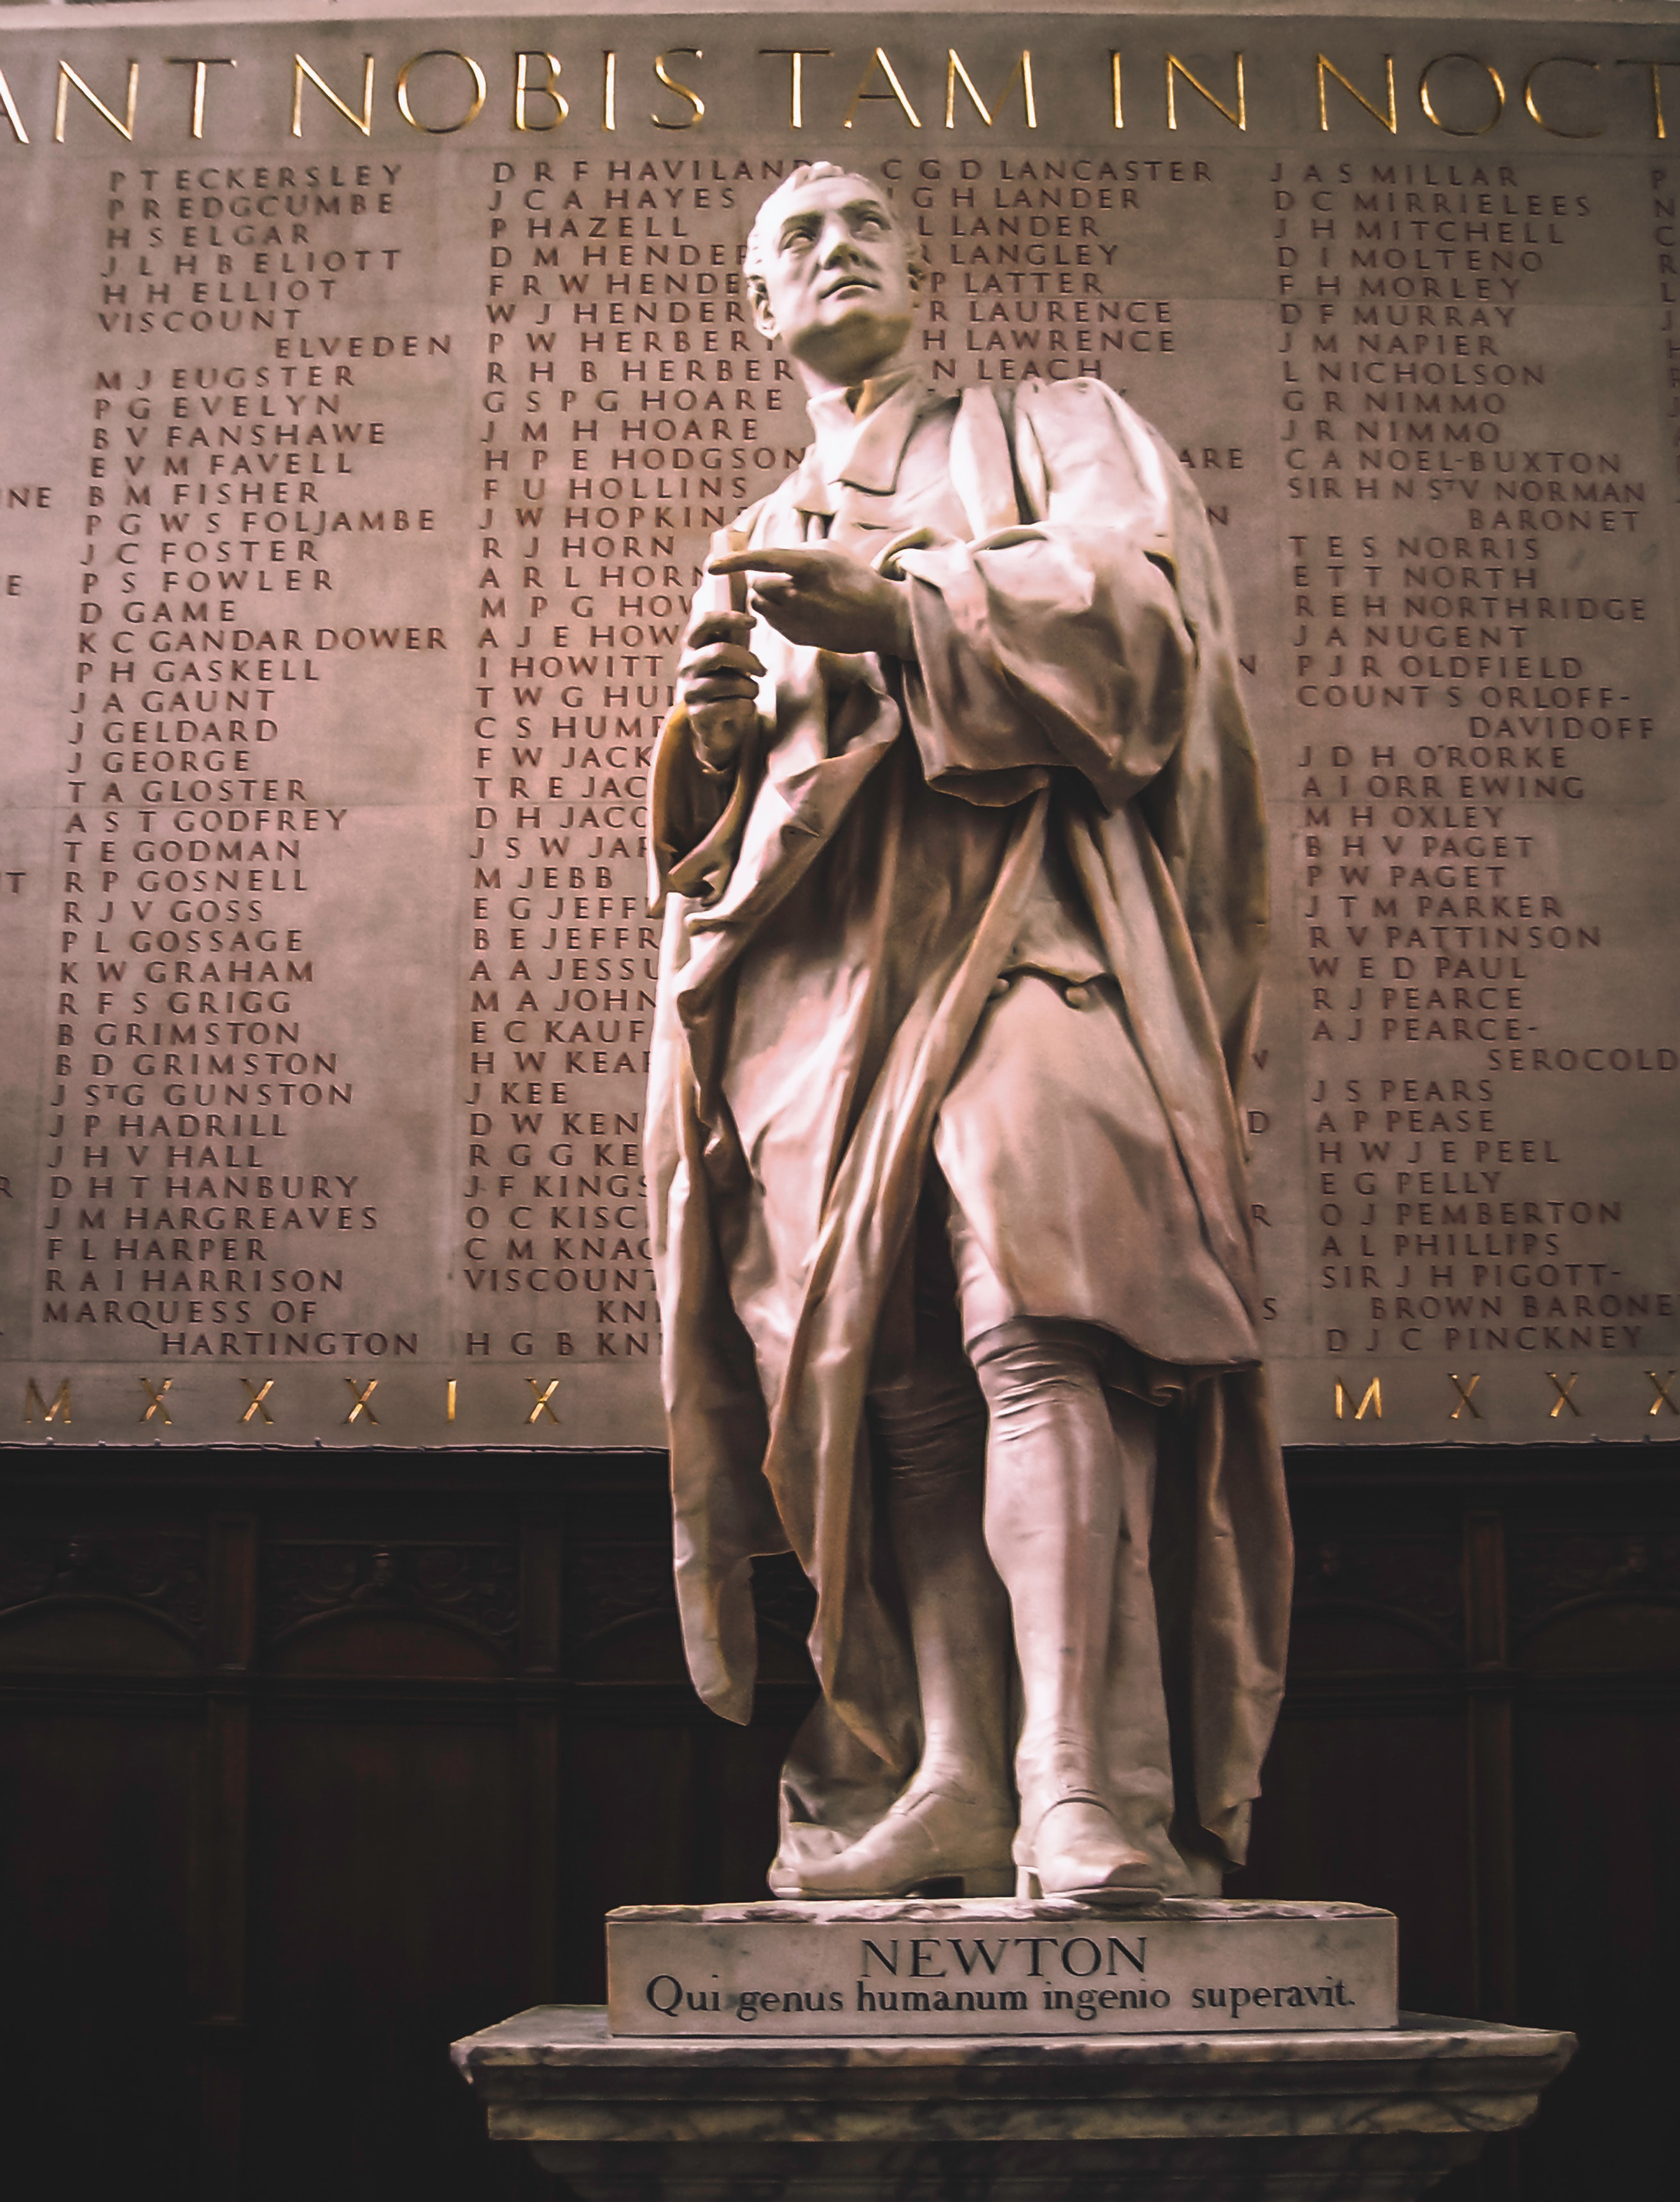
\includegraphics[width=80mm]{./images/NEWTON}}
%        \caption{Geschwindigkeit als Funktion der Zeit}
        \label{fig:Einstein}
    \end{center}
\end{figure}
\newpage

\tableofcontents



\newpage
\newpage
\section {Zusammenfassung}
\subfile{subfiles/Zusammenfassung}
\newpage
\section {Aufbau des Experiments}
\subfile{subfiles/AufbauDesExperiments}
\newpage
\section {Physikalische Beschreibung der einzelnen Vorgänge}
\subfile{subfiles/PhysikalischeBeschreibung}
\newpage
\section {Beschreibung der Implentierung inklusive Screenshots aus Unity}
\subfile{subfiles/Beschreibung der Implentierung inklusive Screenshots aus Unity}
\newpage
\section {Resultate mit grafischer Darstellung}
\subfile{subfiles/ResultateMitGrafischerDarstellung.tex}
\newpage
\section {Rückblick und Lehren aus dem Versuch}
\subfile{subfiles/Rueckblick und Lehren aus dem Versuch}
\newpage


\appendix
\section {Anhang}
\subfile{subfiles/code}

\newpage
\listoffigures

\newpage

\printbibliography


\end{document}